% ----------------------------------------------------------------------------
%
%                           Concrete
%                                Structures
%                                   Summary
%
% ----------------------------------------------------------------------------
%
%

\documentclass[landscape]{article}
\usepackage{kpfonts}
\usepackage{array}
\usepackage{amsmath,amssymb}
\usepackage{booktabs}
\usepackage{caption}
\usepackage[nodayofweek]{datetime}
\usepackage{environ}
\usepackage{float}
\usepackage{enumitem}
\usepackage{fancyhdr}
\usepackage[landscape,margin=13mm,footskip=1pt,includefoot]{geometry}
\usepackage{graphicx}
\usepackage{hyperref}
\usepackage{multicol}
\usepackage{rotating}
\usepackage{tikz}
\usepackage{threeparttable}
\usepackage{url}
\usepackage{xspace}
\usepackage{mathabx}
\usepackage{footnote}
\usepackage{mathtools}
\usepackage[backend=biber]{biblatex}
\addbibresource{./literature.bib}

\usepackage{custom}
\newcommand{\version}{0.2}


% Move footnotes to the bottom-right corner
\pagestyle{fancy}
\fancyhf{} % clear all header and footer fields
\fancyhead{}
\fancyfoot[R]{\footnotesize \thepage}
\renewcommand{\headrulewidth}{0pt}

% Further document tweaks.
\parindent=0pt
\setitemize{itemsep=0.2mm,parsep=1pt}
\setenumerate{itemsep=0.2mm,parsep=1pt}

% A type of blue that doesn't look as aggressive as the default 'blue' but also
% distinguishes well from black while not appearing to light.
\definecolor{trueblue}{rgb}{0.0, 0.45, 0.81}

% Link style (hyperref package)
\hypersetup{
  colorlinks=true,        % false: boxed links; true: colored links
  linkcolor=black,        % color of internal links
  citecolor=trueblue,     % color of links to bibliography
  filecolor=trueblue,     % color of file links
  urlcolor=trueblue       % color of external links
}


% An itemize list with a title that avoids a break between title and list.
\newenvironment{titemize}[1]{
  \begin{minipage}[h]{\columnwidth}
    #1
    \begin{itemize}
}{
    \end{itemize}
  \end{minipage}
}

\begin{document}

\thispagestyle{empty}
\begin{center}
  \vspace*{\fill}
  \textsc{\Huge Concrete Structures\\[2ex] \huge Summary}
  \vfill
  \footnotesize{
    Version \version\\[1ex]
    \today\\[1ex]
    Github \copyright{}
    \href{https://github.com/mbataillou?tab=repositories}{Marc Bataillou Almagro}\\
  }
\end{center}
\newpage

\thispagestyle{empty}
\begin{multicols*}{3}
  \tableofcontents
\end{multicols*}
\newpage

\begin{multicols*}{2}

\section{General} % (fold)
\label{sec:general}
    $$
      \begin{aligned}
        & KPa = \frac{KN}{m^2} \Leftrightarrow MPa = \frac{N}{mm^2} \\
        & I_c= I_{rectangle} = \frac{bd^3}{12} \\
        & I_{circle}= \frac{\pi R^4}{4}= \frac{\pi D^4}{64}\\
        & I_{G+x} = I_G + Ax^2 \emph{ Steiner (x perpendicular to the ref axis)}
      \end{aligned}\notag
    $$


\section{Inertia} % (fold)
\label{sec:inertia}
    \subsection{Before cracking} % (fold)
    \label{sub:before_cracking}
    
\begin{multline}
  I = \sum_{i=1}^n \alpha_i\left[I_i + A_i (y_i-\bar{y})^2\right]=\\ I_c + A_c \left(y_c-\bar{y}\right)^2 + \alpha\left[I_s + I_s^t + A_s \left(y_s-\bar{y}\right)^2 + A_s^t (y_s^t-\bar{y})^2\right] 
\end{multline}

  where
    $$
      \begin{aligned}
        &\bar{y}= \frac{\sum y_i A_i \alpha_i  }{\sum  A_i \alpha_i} = \frac{y_c A_c + y_s A_s \alpha + y_s^t A_s^t \alpha  }{ A_c +  A_s \alpha +  A_s^t \alpha} \\
        & \alpha_i = \frac{E_i}{E_j} = \alpha = \frac{E_s}{E_c}
      \end{aligned}\notag
    $$


    \subsubsection{Aproximation} % (fold)
    \label{ssub:aproximation}
    $$
      \begin{aligned}
        &I_{gross}= \frac{bd^3}{12} \approx 0.9 I \\
        & E_c = 22\left(\frac{f_{ck}+8}{10}\right)^{0,3}
      \end{aligned}\notag
    $$

    % subsubsection aproximation (end)

    \subsection{Cracked} % (fold)
    \label{sub:cracked}

    \begin{multline}
      I = \sum_{i=1}^n \alpha_i[I_i + A_i (y_i-x)^2]=\\ I_c + A_c (y_c-x)^2 + \alpha[I_s + I_s^t + A_s (y_s-x)^2 + A_s^t (y_s^t-x)^2]  
    \end{multline}

  where
    $$
      \begin{aligned}
        &\frac{x_{cracked}}{d}= \alpha \rho \left(1 + \frac{\rho^t}{\rho} \right) \left[ - 1 \sqrt{1+ \frac{2\left(1 + \frac{d^t\rho^t}{d\rho}\right)}{\alpha \rho \left(1 + \frac{\rho^t}{\rho}\right) } }\right] \\
        & I_c= I_{rectangle/bottom} = \frac{bd^3}{3}
      \end{aligned}\notag
    $$

    \subsubsection{Approximation} % (fold)
    \label{ssub:approximation}

    \begin{gather}\label{eq:2.1}
      I \approx \frac{bd^3}{3}+ \alpha[ A_s (y_s-x)^2 + A_s^t (y_s^t-x)^2] \\
      \shortintertext{where}
      \begin{aligned}
        &\frac{x_{cracked}}{d} \approx \frac{0.18 + 1.8\alpha \rho }{1 + \frac{d^t \rho^t }{d \rho}}
      \end{aligned}\notag
    \end{gather}

\section{Material deformation} % (fold)
    \label{sec:material_properties}
    \begin{enumerate}
      \item Elastic deformation

      \begin{gather}\label{eq:2.1}
      \varepsilon_i(t_1) = \frac{\sigma(t_1) }{E_c (t_1)} \\
      \shortintertext{where}
      \begin{aligned}
        & \sigma(t_1): \emph{ is the tension at $t_1$} \\
        & E_c (t_1): \emph{ is the elastic modulus at $t_1$}
      \end{aligned}\notag
      \end{gather}

      \item Creep 
        \begin{gather}\label{eq:2.1}
        \varepsilon_{cc}(t_2,t_1) = \varphi(t_2,t_1) \frac{\sigma(t_1) }{E_c (28)} \\
        \shortintertext{where}
        \begin{aligned}
          & \varphi(t_2,t_1): \emph{ is the creep coeficient from $t_1$ to $t_2$ see material \textsc{PP}} \\
          & \varphi(\infty,t_1): \emph{ see Figures~\ref{fig:creep_infinity_1},\ref{fig:creep_infinity_2}}
        \end{aligned}\notag
        \end{gather}

      \item Shrinkage

        \begin{gather}\label{eq:2.1}
        \varepsilon_{cs}=\varepsilon_{ca}+\varepsilon_{cd} \\
        \shortintertext{where}
        \begin{aligned}
          & \varepsilon_{ca}= 
          \begin{cases}
            \varepsilon_{ca}= \beta_{as}(t) \varepsilon_{ca}(\infty)\\
            \beta_{as}(t)= 1- e^{-0.2t^{0.5}} \\
            \varepsilon_{ca}(\infty) =2.5(f_{ck}-10)\cdot 10^{-6} 
          \end{cases}\emph{ is the autogenous shrinkage} \\
          & \varepsilon_{cd} =
          \begin{cases}
            \varepsilon_{cd}= \beta_{ds}(t,t_s)k_h \varepsilon_{cd,0}\\
            \beta_{ds}(t,t_s)= \frac{t-t_s}{t-t_s + 0.04   \sqrt{h_0^3} }
        \end{cases} \emph{ is the drying shrinkage} \\
        & h_0 \emph{ is the shape coefficient} \\
        & k_h \emph{ see Table~\ref{tab:k_h}}
        \end{aligned}\notag
        \end{gather}
\end{enumerate}

    \begin{figure}[H]
        \centering
        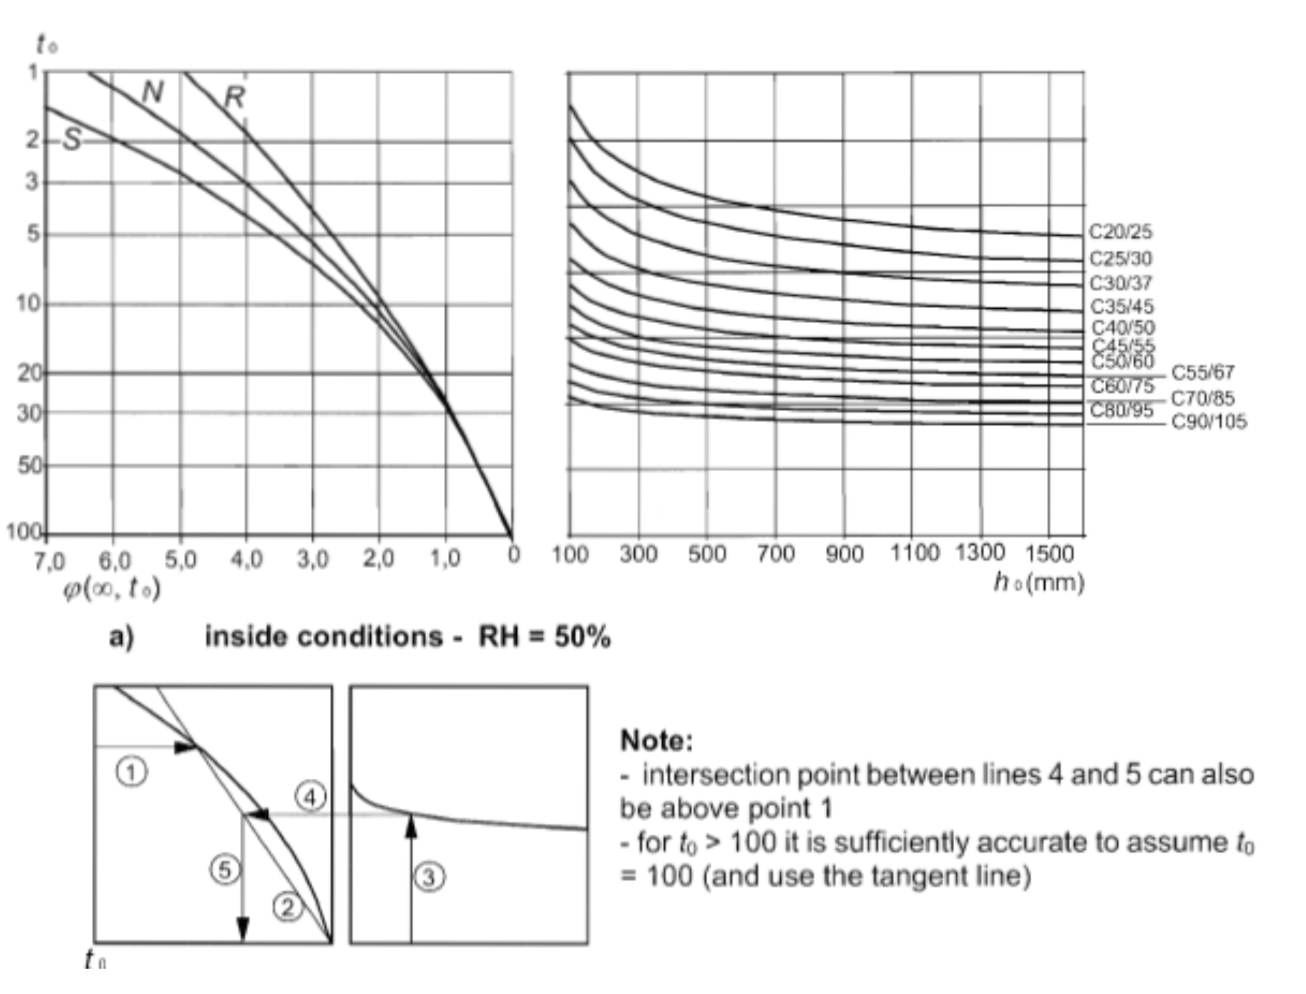
\includegraphics[width=0.95\linewidth]{img/phi1}
        \caption{Model for infinite creep coefficient RH =50}
        \label{fig:creep_infinity_1}
    \end{figure}

    \begin{figure}[H]
        \centering
        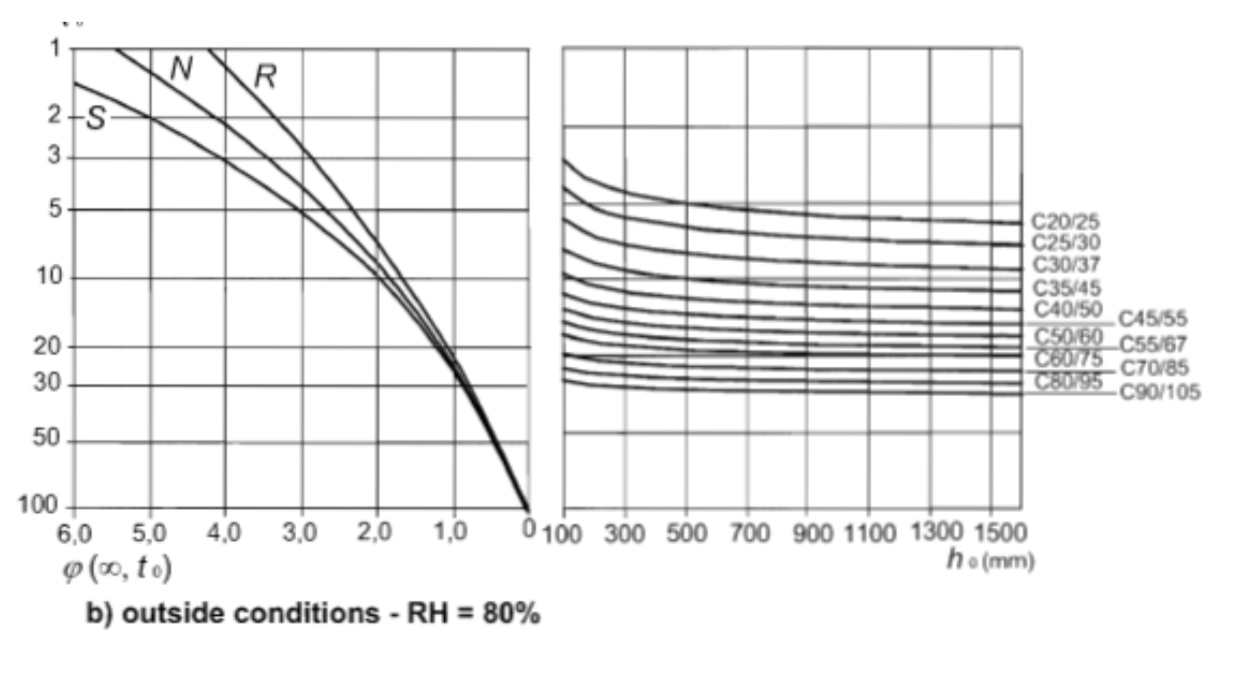
\includegraphics[width=0.95\linewidth]{img/phi2}
        \caption{Model for infinite creep coefficient RH =80}
        \label{fig:creep_infinity_2}
    \end{figure}

    \begin{table}[H]
    \centering
        \begin{tabular}{cc}
            \toprule
            $h_0$ & $k_h$\tabularnewline
            \midrule
            100 & 1\tabularnewline
            
            200 & 0.85\tabularnewline
            
            300 & 0.75 \tabularnewline
            
            $\leq 500$ & 0.7\tabularnewline
            \bottomrule
        \end{tabular}
        \caption{$k_h$ depending on $h_0$}
        \label{tab:k_h}
    \end{table}

    % section material_properties (end)

% section longitudinal_reinforcement (end)

\section{Durability requirements} % (fold)
\label{sec:durability_requirements}
\begin{enumerate}
  \item Find exposure class in Table~\ref{tab:expo_class}
  \item Define concrete class with Table~\ref{tab:concrete_class}
  \item Compute structural class with Table~\ref{tab:struct_class}, taking into account that $S_{min} =S_1$ and $S_{ref,T=50y}=S_4$
  \item Find minimal cover in Table~\ref{tab:min_cover}
  \item Add tolerance
  \[
    C_{dur} = C(Table~\ref{tab:min_cover}) + \Delta c 
  \]
   \begin{gather}\label{eq:2.1}
        C_{dur} = C(Table~\ref{tab:min_cover}) + \Delta c  \\
        \shortintertext{where}
        \begin{aligned}
          & \Delta c \in [0,10] \rightarrow 5mm 
        \end{aligned}\notag
        \end{gather}
\end{enumerate}

\begin{table}[H]
    \centering
    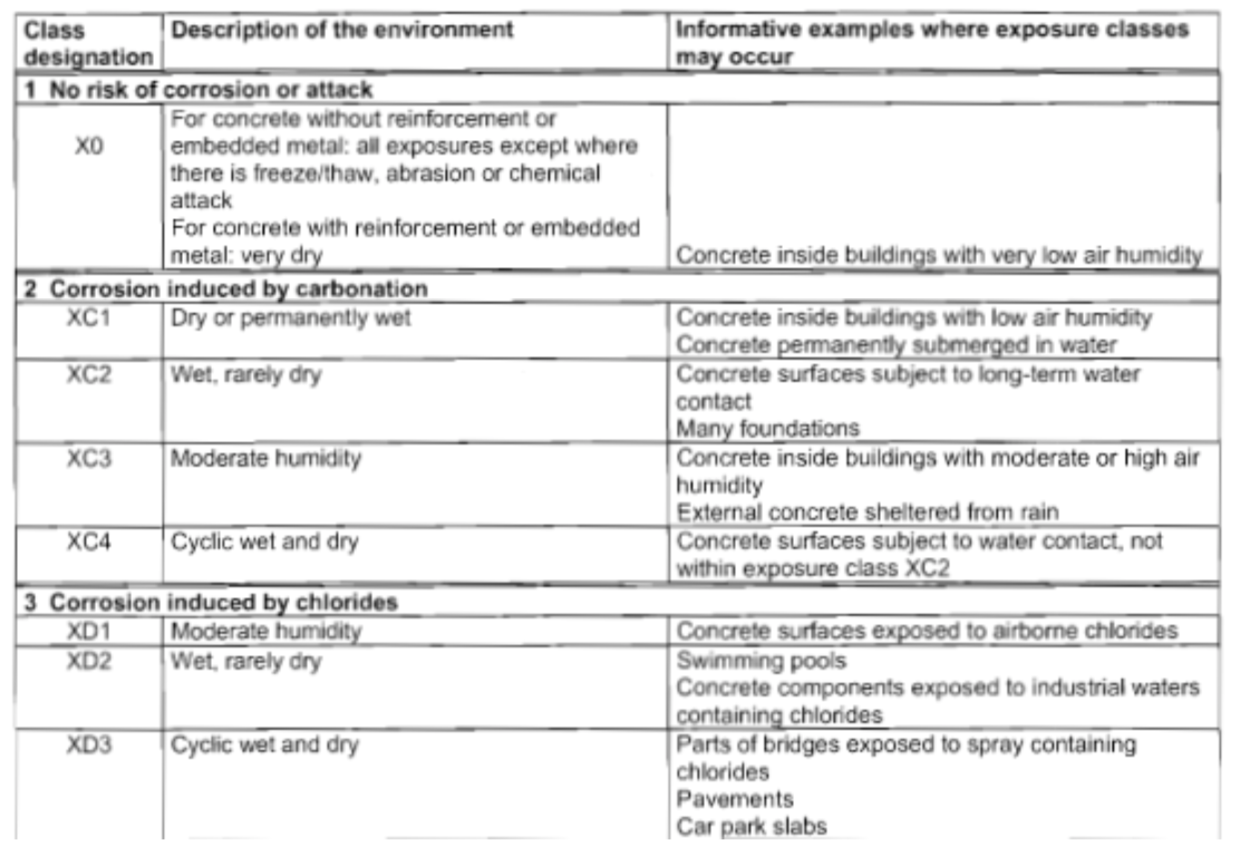
\includegraphics[width=0.95\linewidth]{img/expo_class}\\
    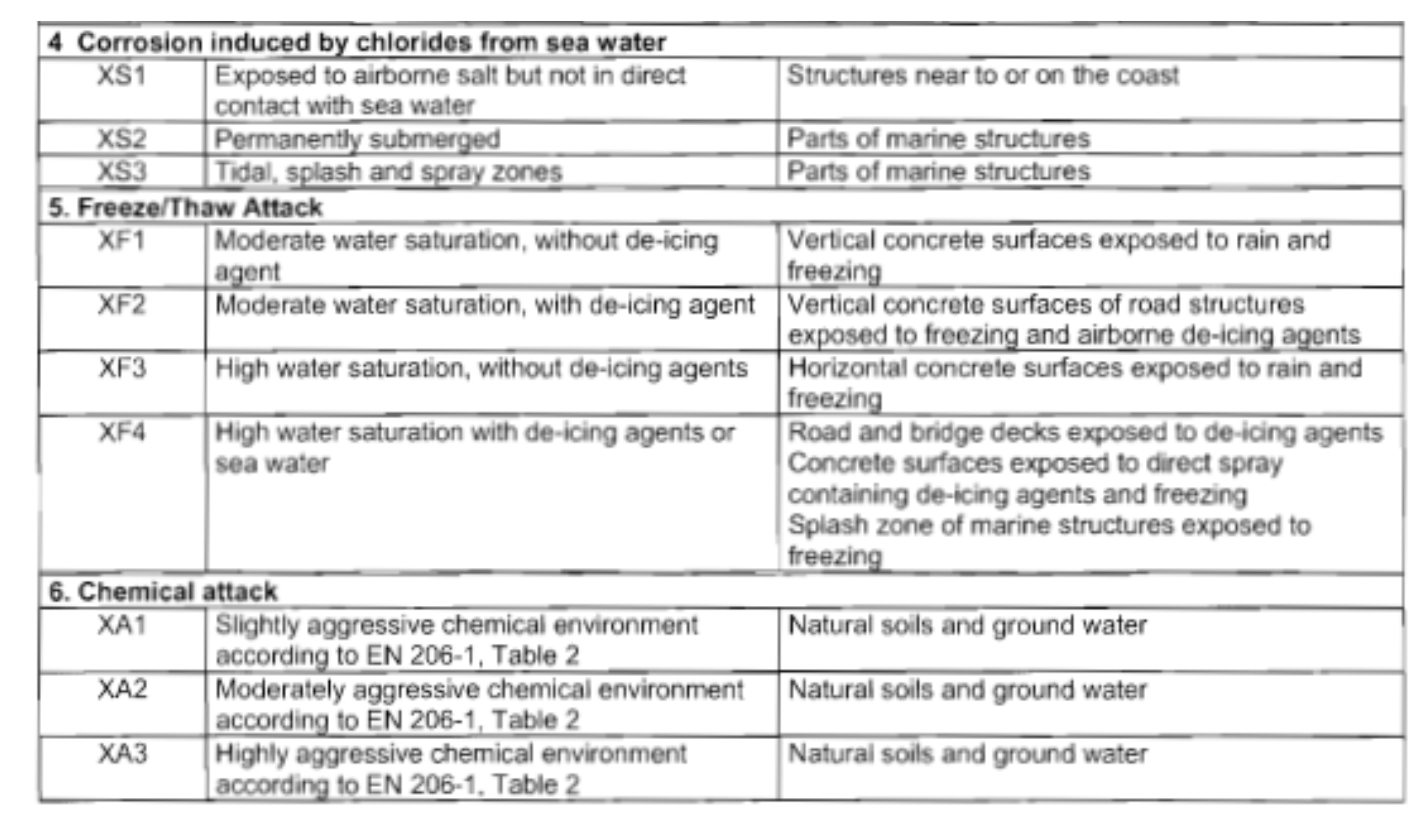
\includegraphics[width=0.95\linewidth]{img/4_1.png}
    \caption{Exposure class}
    \label{tab:expo_class}
\end{table}

\begin{table}[H]
    \centering
    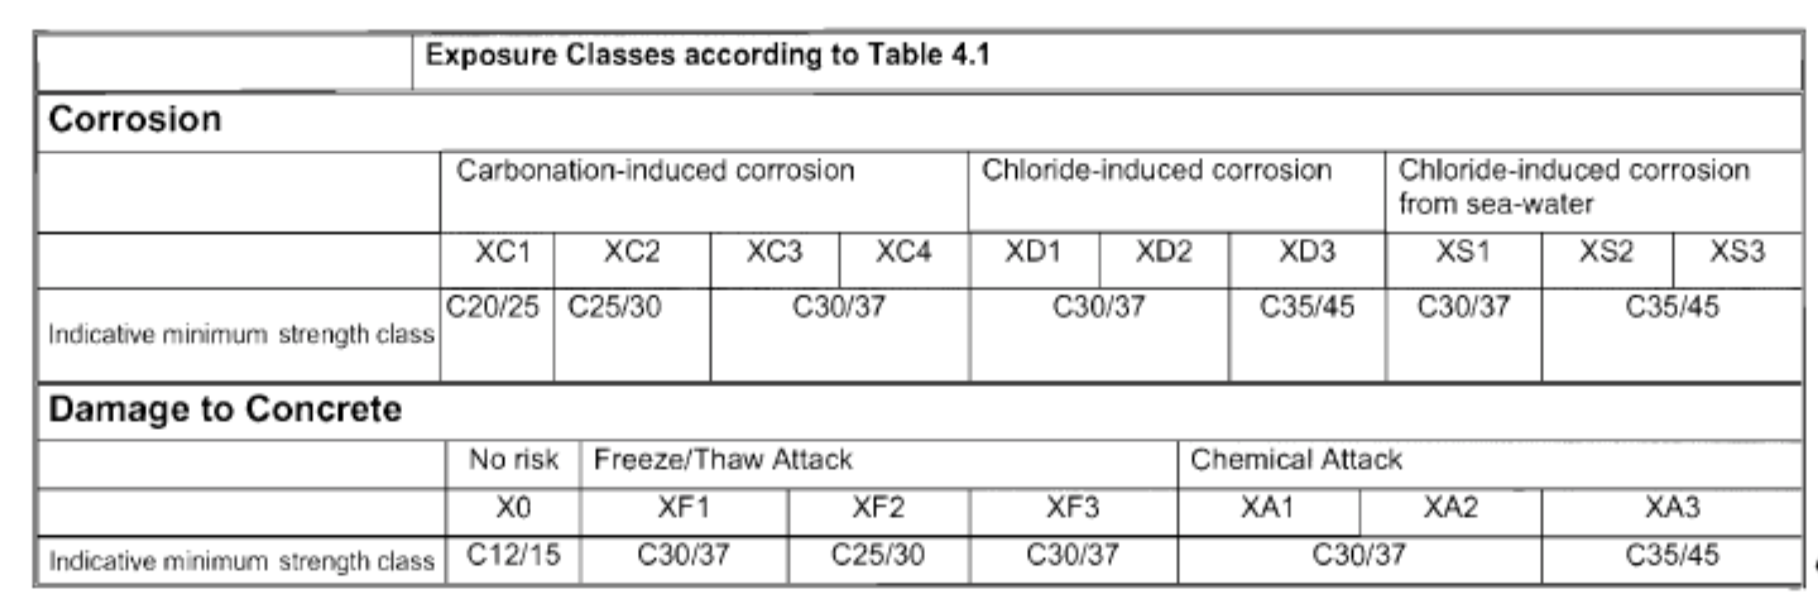
\includegraphics[width=0.95\linewidth]{img/min_class.png}
    \caption{Concrete class depending on exposure class}
    \label{tab:concrete_class}
\end{table}

\begin{table}[H]
    \centering
    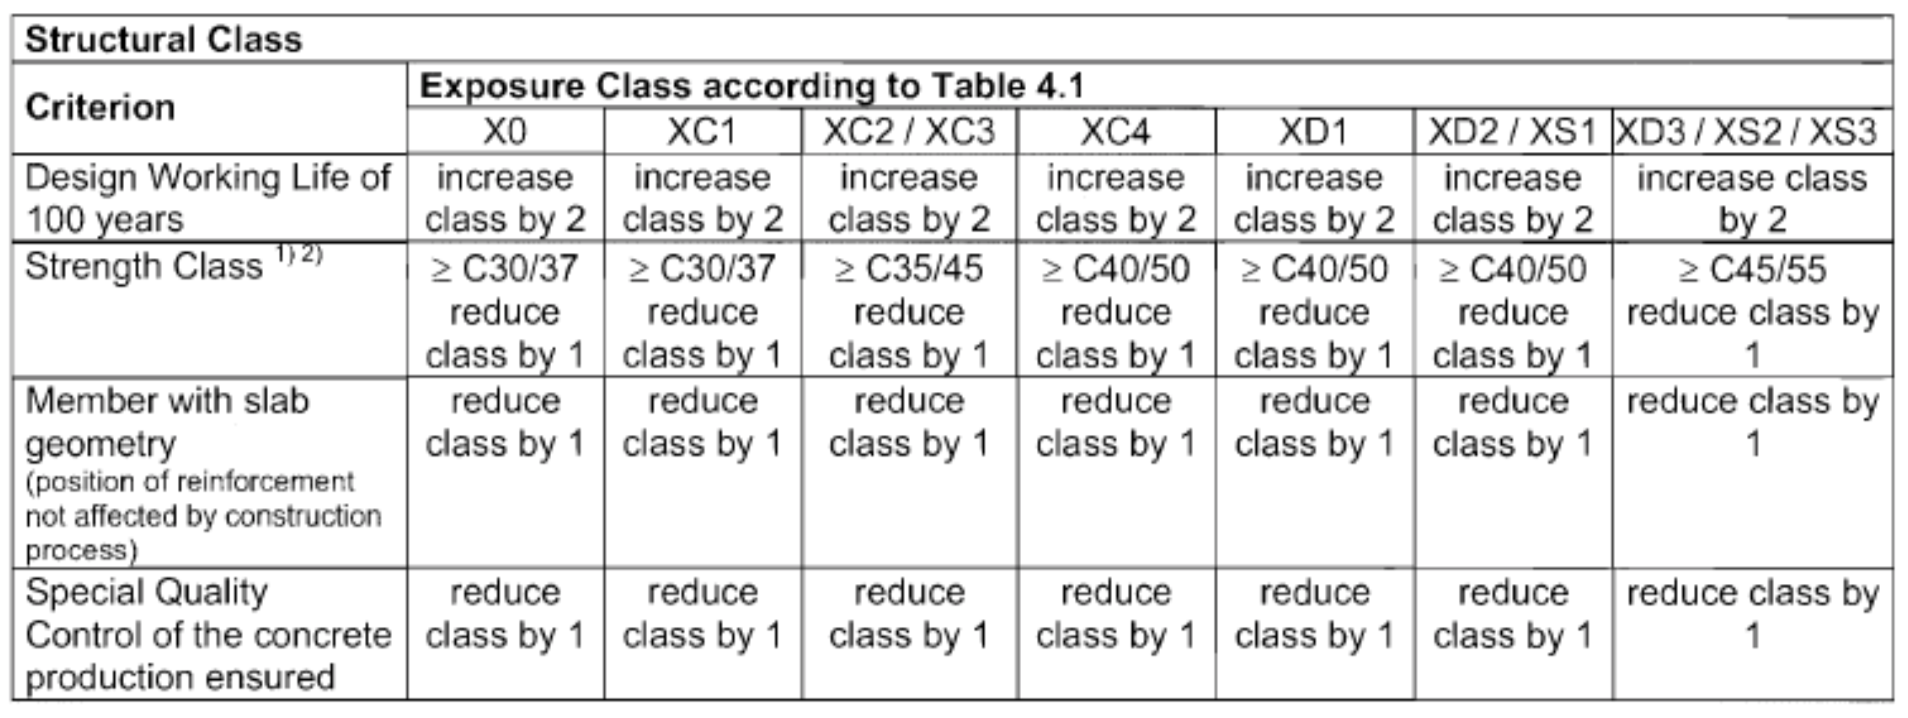
\includegraphics[width=0.95\linewidth]{img/4_3.png}
    \caption{Structural class}
    \label{tab:struct_class}
\end{table}
\begin{table}[H]
    \centering
    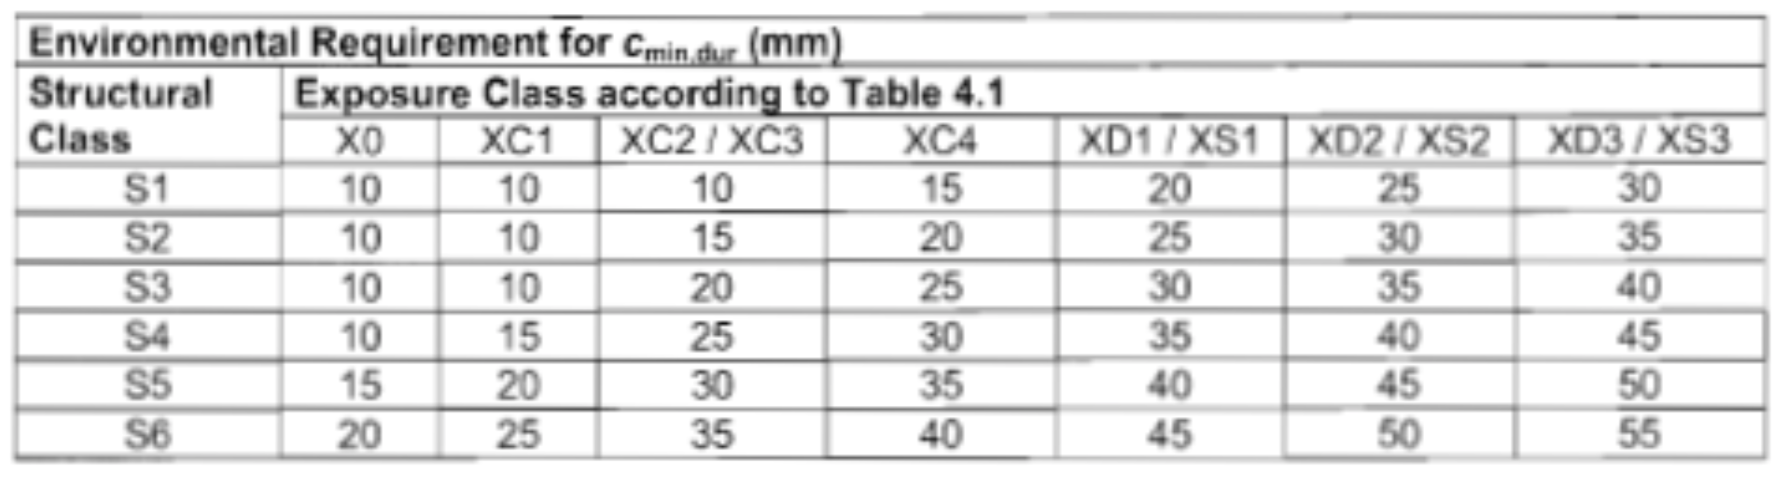
\includegraphics[width=0.95\linewidth]{img/4_4.png}
    \caption{Minimal required cover depending on exposure and structural class}
    \label{tab:min_cover}
\end{table}

% section durability_requirements (end)

\section{Load combinations} % (fold)
\label{sec:load_combinations}
\subsection{Ultimate limit state} % (fold)
\label{sub:ultimate_limit_state}
\begin{gather}\label{eq:2.1}
      \sigma_{ULS} = \gamma_G \sum G_i + \gamma_P P + \gamma_Q Q_1+ \gamma_Q \psi_0\sum_{i\neq 1} Q_i  \\
      \shortintertext{where}
      \begin{aligned}
        &\gamma_G = 1,35: \emph{ is the security factor for permanent loads} \\
        &\gamma_Q = 1,5: \emph{ is the security factor for live loads} \\
        &\gamma_P: \emph{ is the security factor for prestressing load} \\
        &\psi_0 : \emph{ is a factor accounting for the frequence (probability)}\\
        &Q_1: \emph{ is the principal live load}\\
        &Q_i \ i \neq 1: \emph{ is a secondary live load} \\
        &G_i: \emph{ is a permanent load}
      \end{aligned}\notag
    \end{gather}
\subsection{Service state} % (fold)
\label{sub:service_state}
\begin{itemize}[label=\ding{69}]
  \item Characteristic
  \begin{gather}\label{eq:2.1}
      \sigma_{CHA} = \sum G_i + P + Q_1+ \psi_0\sum_{i\neq 1} Q_i  \\
  \end{gather}
  \item Frequent
    \begin{gather}\label{eq:2.1}
      \sigma_{FRE} = \sum G_i + P + \psi_1Q_1+ \psi_2\sum_{i\neq 1} Q_i  \\
      \shortintertext{where}
      \begin{aligned}
        &\psi_1 : \emph{ is a factor accounting for the frequence (probability)}\\
        &\psi_2 : \emph{ is a factor accounting for the frequence (probability)}
      \end{aligned}\notag
  \end{gather}
  \item Quasi-permanent
  \begin{gather}\label{eq:2.1}
      \sigma_{QUA} = \sum G_i + P + \psi_2\sum Q_i  \\
  \end{gather}
\end{itemize}
% subsection service_state (end)
% subsection ultimate_limit_state (end)

% section load_combinations (end)

\section{Longitudinal reinforcement} % (fold)
\label{sec:longitudinal_reinforcement}
\subsection{Aproximations} % (fold)
\label{sub:aproximations}
\subsubsection{Design} % (fold)
\label{ssub:design}
\[
  d \approx 0,9h
\]
\begin{enumerate}
  \item if $fyk = 400$
  \begin{gather}\label{eq:2.1}
        M_{lim} \approx 0,369 f_{cd} bd^2 \\
        x_{lim} \approx 0,668 d \\
        y_lim \approx 0,534 d
        \shortintertext{where}
        \begin{aligned}
          &M_{lim}: \emph{ is the max moment resisted without comp reinforcement} \\
          &x_{lim}: \emph{ is the x where steel starts yielding} \\
          &y_{lim}: \emph{ is the effective comp zone}
        \end{aligned}\notag
  \end{gather}
  \item if $fyk = 500$
  \begin{gather}\label{eq:2.1}
        M_{lim} \approx 0,375 f_{cd} bd^2 \\
        x_{lim} \approx 0,617 d \\
        y_{lim} \approx 0,5 d
  \end{gather}
  \end{enumerate}
% subsection aproximations (end)
\subsection{Spacing} % (fold)
\label{sub:spacing}
\begin{enumerate}
  \item Define $\phi_l$, see Table~\ref{tab:diam_long}
  \item Compute $n = \frac{A_s}{\frac{\phi^2}{4}}$
  \item Compute
    \begin{gather}\label{eq:2.1}
      s = \frac{b - 2c - 2\phi_t - n\phi_l}{n-1} \\
      \shortintertext{where}
      \begin{aligned}
        &s > \max(30mm (1,25 \cdot \phi_{arid}); \phi_{long})
        &b: \emph{ is the width} \\
        &c: \emph{ is the minimal cover} \\
        &\phi_t: \emph{ is the transversal reinforcement diameter}
      \end{aligned}\notag
    \end{gather}
\end{enumerate}

\begin{table}[H]
\centering
  \begin{tabular}{cc}
  \toprule
  Diameter [$mm$]& Area [$mm^2$] \\
  \midrule
  12 & 113 \\
  (14) & 154 \\
  16 & 200 \\
  20 & 314 \\
  25 & 490 \\
  \bottomrule
  \end{tabular}
  \caption{Common diameters for longitudinal reinforcement}
  \label{tab:diam_long}
\end{table}

% subsection spacing (end)
\subsection{Optimisation} % (fold)
\begin{enumerate}
  \item Choose reduction factor $n$
  \item Find $x$ where $M_{d,x} = nM_d$
  \item if $\sigma_s\neq f_{yd}=435MPa$Compute 
  \begin{gather}\label{eq:2.1}
      l_{b,rqd} = l_{table} \frac{\sigma_s}{f_{yd}} \\
      \shortintertext{where}
      \begin{aligned}
        &l_{table}: \emph{ see Table~\ref{tab:l_table}} 
      \end{aligned}\notag
    \end{gather}
  \item else $l_{b,rqd} = l_{table}$
  \item Apply correction for layout
  \begin{enumerate}
    \item Anchoring
  \begin{gather}\label{eq:2.1}
      l_0 =  l_{b,rqd}\Pi_{i=1}^5 \alpha_i \approx k l_{b,rqd} \\
      \shortintertext{where}
      \begin{aligned}
        &\alpha_i: \emph{ see Figures~\ref{fig:alpha}\ref{fig:c_d}} \\
        & k = 
        \begin{cases}
          1 &\text{ if } \emph{straight}\\
          0,7 &\text{ if } \emph{hook}
        \end{cases}
      \end{aligned}\notag
    \end{gather}
    \begin{gather}\label{eq:2.1}
      l_0 = \max(l_0,l_{b,min}) \\
      \shortintertext{where}
      \begin{aligned}
        &l_{b,min}: \emph{ see Table~\ref{tab:l_min}} 
      \end{aligned}\notag
    \end{gather}

    \item Connecting
    \begin{gather}\label{eq:2.1}
      l_0 =  l_{b,rqd}\Pi_{i=1, i\neq 4}^6 \alpha_i \\
      \shortintertext{where}
      \begin{aligned}
        &\alpha_i, i\neq3: \emph{ see Figure~\ref{fig:alpha}}\\
        &  \alpha_3: \sum A_{s,min} = A_s \frac{\sigma_{sd}}{f_{yd}}, \quad A_s \emph{ the area of one lapped bar}\\
        & \emph{See more details in PP}
      \end{aligned}\notag
    \end{gather}
    \begin{gather}\label{eq:2.1}
      l_0 = \max(l_0,l_{min}) \\
      \shortintertext{where}
      \begin{aligned}
        &l_{0,min}= \max(0,3 \alpha_6l_{b,rqd}; 15 \phi ; 200mm )
      \end{aligned}\notag
    \end{gather}
    \end{enumerate}
  \item Cut the bars at $x = x + d + l_{b,rqd}$
\end{enumerate}

\begin{table}[H]
  \centering
  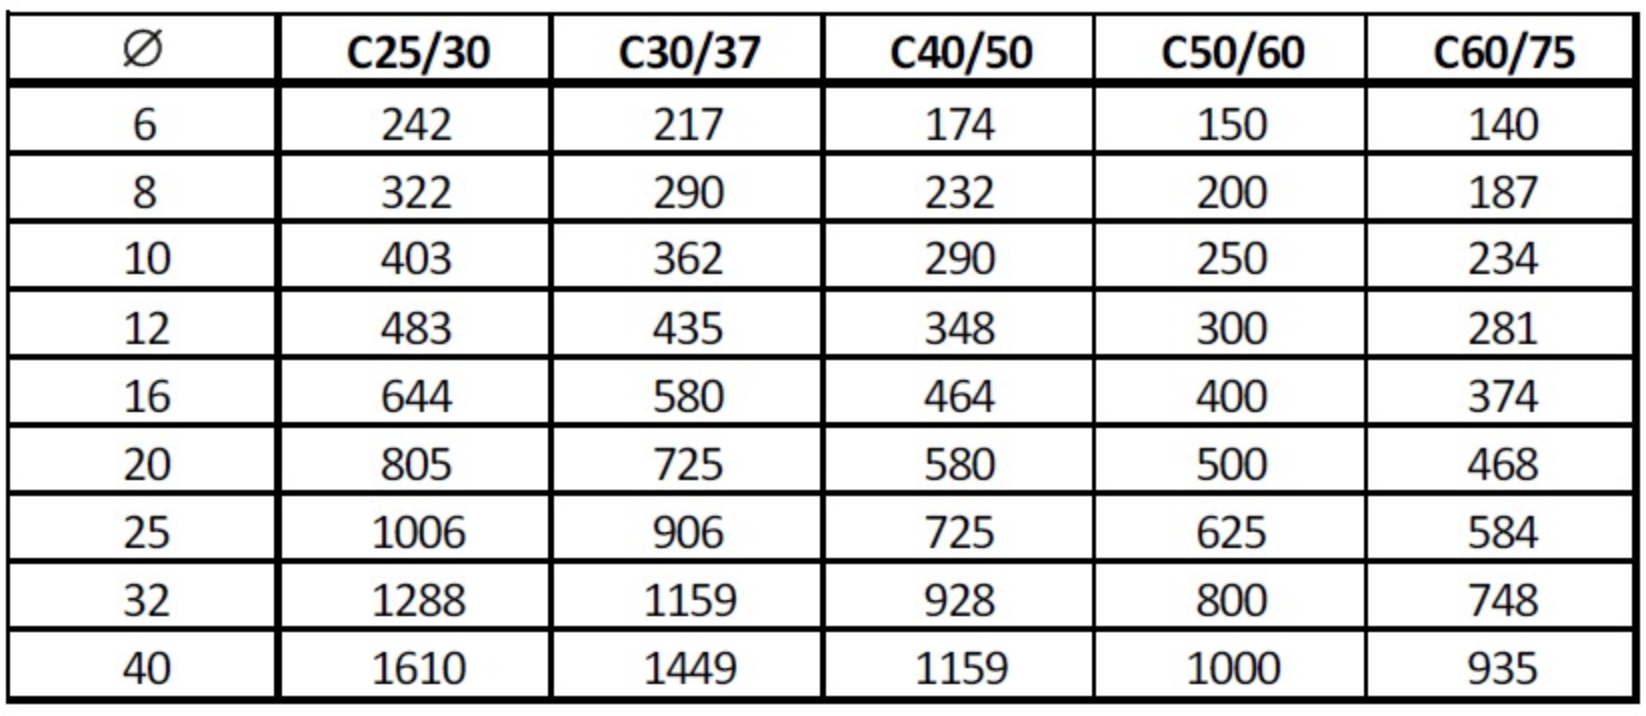
\includegraphics[width = .9\linewidth]{img/l_table.png}
  \caption{$l_{b,rqd}$ for $\sigma_s= f_{yd}=435MPa$}
  \label{tab:l_table}
\end{table}
\begin{table}[H]
  \centering
  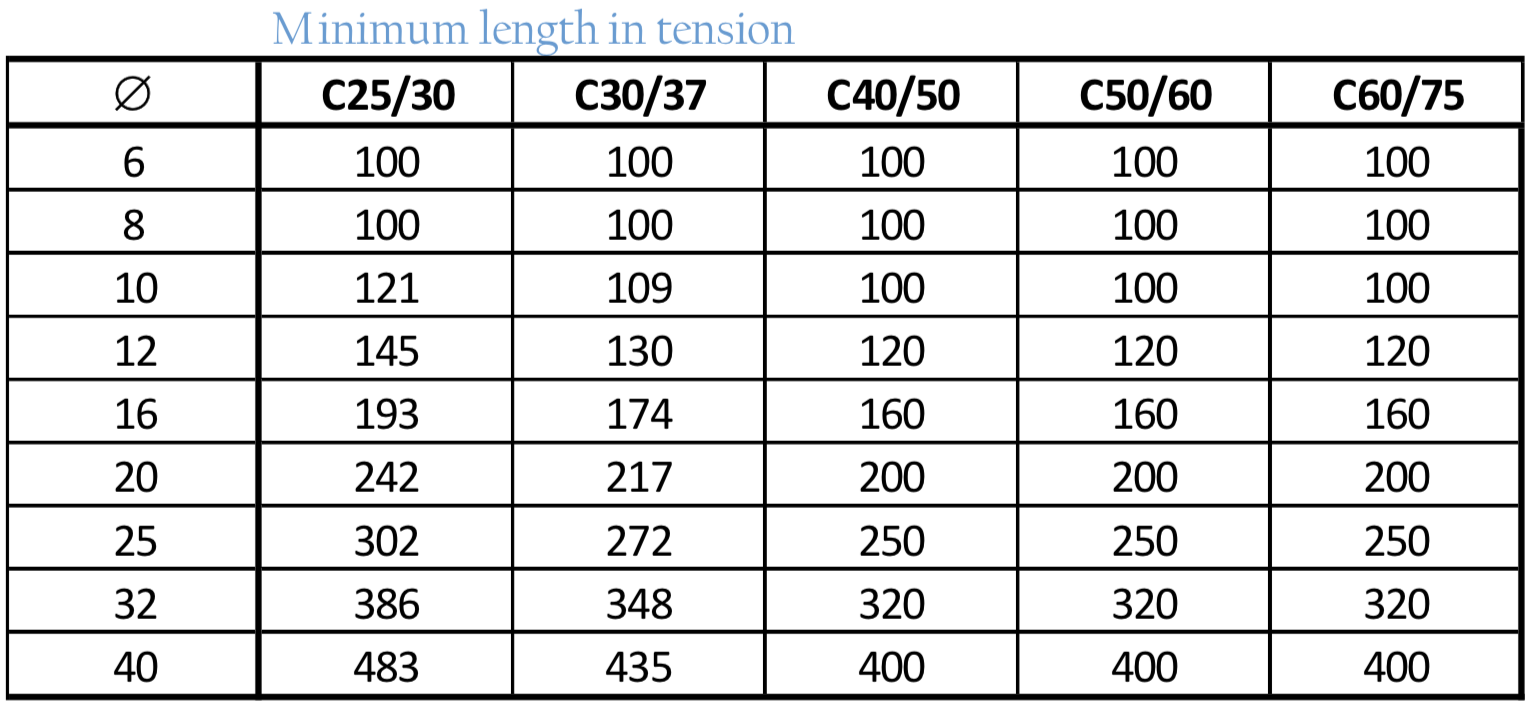
\includegraphics[width = .4\linewidth]{img/l_table_tens.png}
  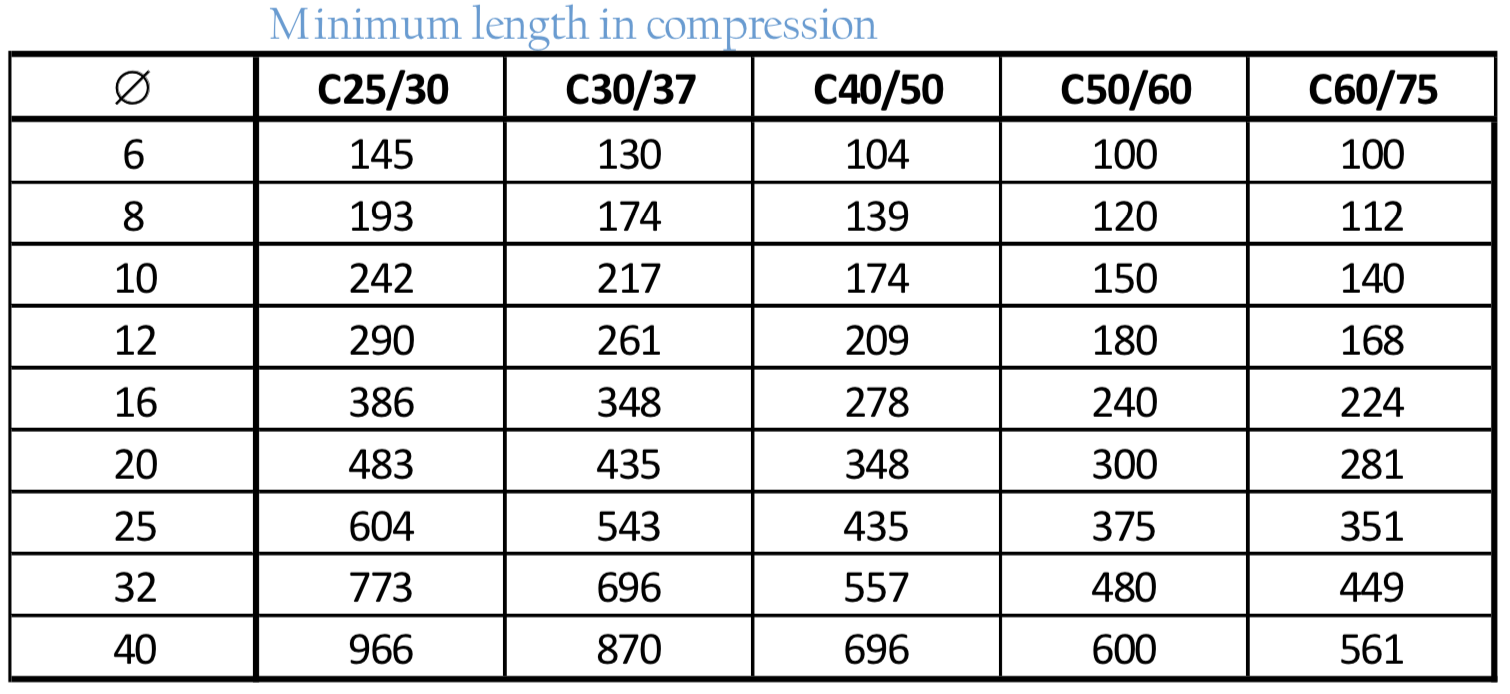
\includegraphics[width = .4\linewidth]{img/l_table_comp.png}
  \caption{$l_{min}$ depending on $\phi$ and $f_{ck}$}
  \label{tab:l_min}
\end{table}
\begin{figure}[H]
  \centering
  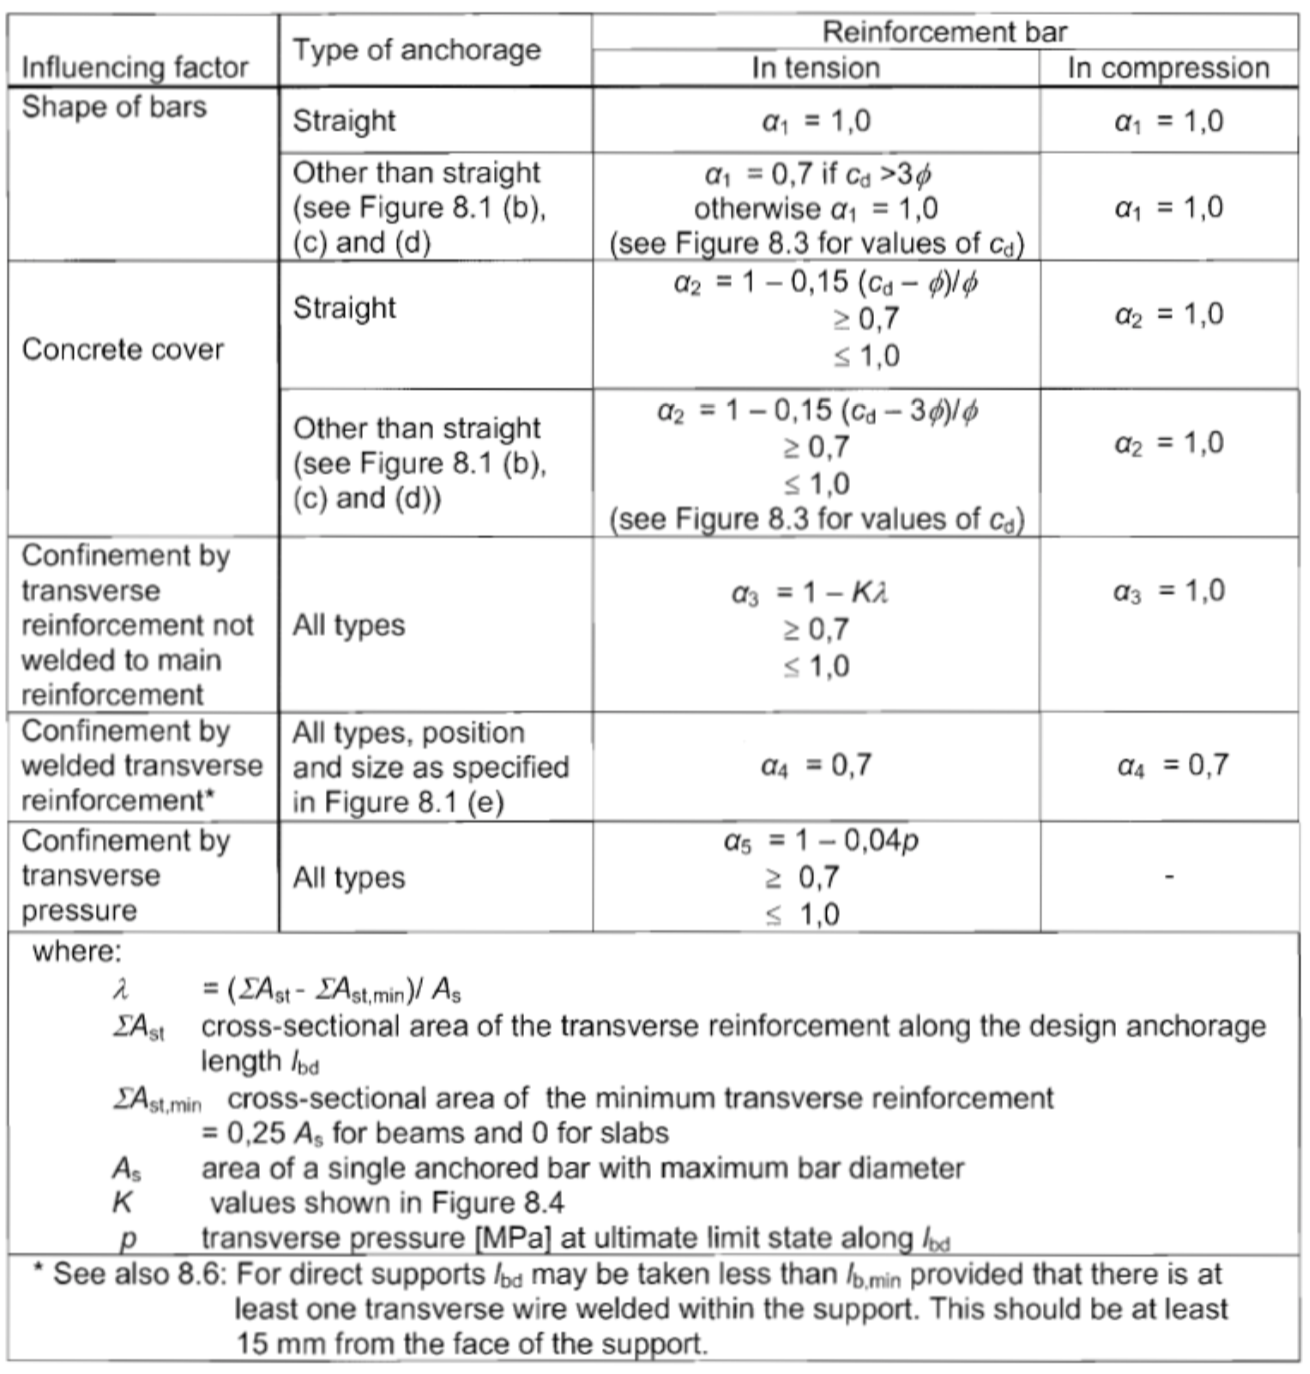
\includegraphics[width = .9\linewidth]{img/alpha.png}\\
  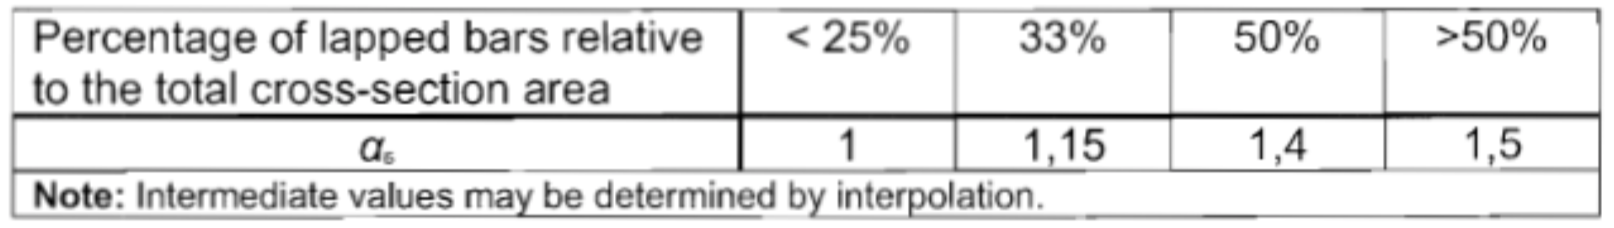
\includegraphics[width = .9\linewidth]{img/alpha_bis.png}
  \caption{$\alpha_i$ depending on the layout}
  \label{fig:alpha}
\end{figure}
\begin{figure}[H]
  \centering
  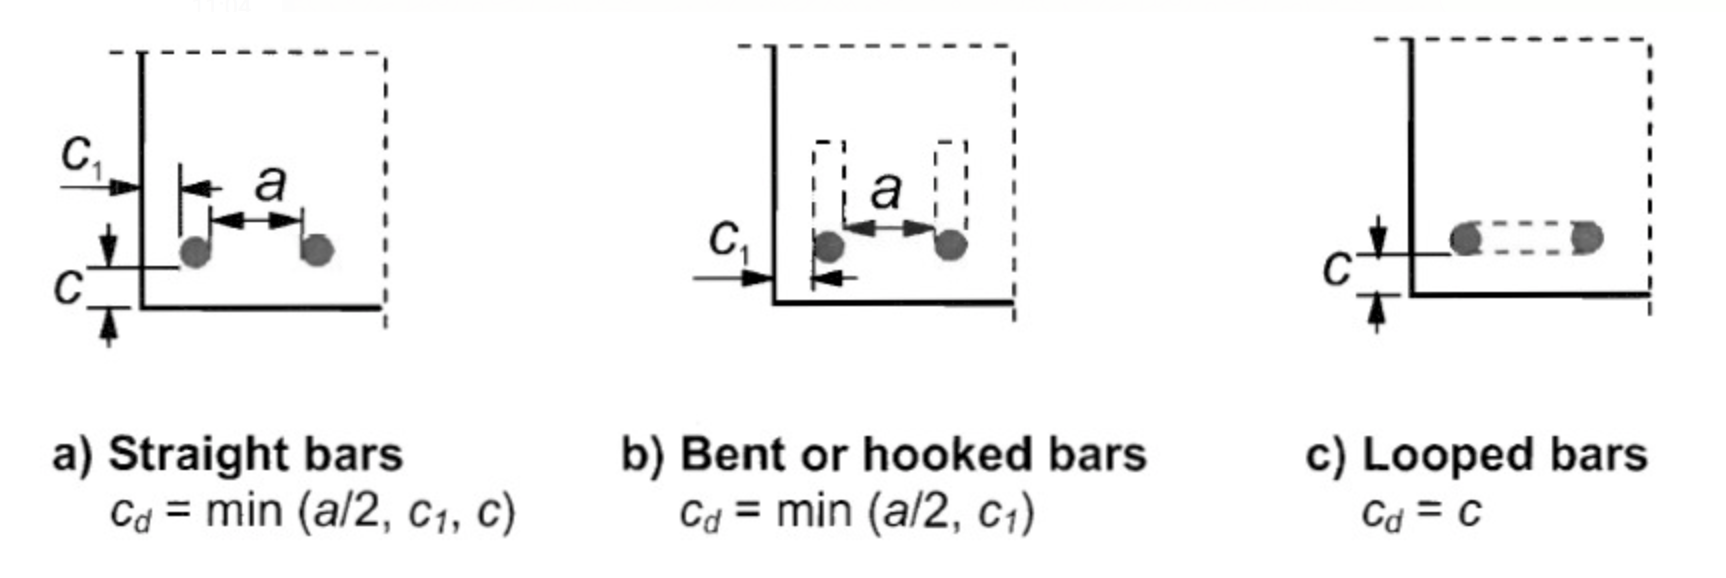
\includegraphics[width = .9\linewidth]{img/c_d.png}
  \caption{$c_d$ depending on the layout}
  \label{fig:c_d}
\end{figure}

% subsection assessment (end)

\section{Crack width control} % (fold)
\label{sec:crack_width_control}
\subsection{Reinforced} % (fold)
\label{sub:reinforced}

\begin{enumerate}
  \item Compute $M_{quasi}$
  \item Compute $x_{cracked}$ see \ref{sub:cracked}
  \item Compute
  \begin{gather}\label{eq:1.4}
        \sigma_s =  \frac{M_{quasi}}{\left(d- \frac{x_{cracked}}{3}\right)A_s}\\
        \shortintertext{where}
        \begin{aligned}
          & d = h - c - \phi_t -k\phi_l\\
          & k: \emph{ is a parameter depending on number of layers}
        \end{aligned}\notag
    \end{gather}
  \item Check allowable crack width in Table~\ref{tab:max_crack}
  \item Compute  $\sigma_{crack} = \max( \sigma (Table~\ref{tab:tension_grieta}), \sigma (Table~\ref{tab:spacing_grieta}))$
  \item If $\sigma_{crack}> \sigma_s$
    \begin{gather}\label{eq:1.4}
        A_{s,crack} = \frac{\sigma_{crack}}{\sigma_s} A_s\\
        \shortintertext{where}
        \begin{aligned}
          & A_{s,crack}: \emph{ is the area needed to fullfill crack width}
        \end{aligned}\notag
    \end{gather}
\end{enumerate}

\begin{table}[H]
    \centering
    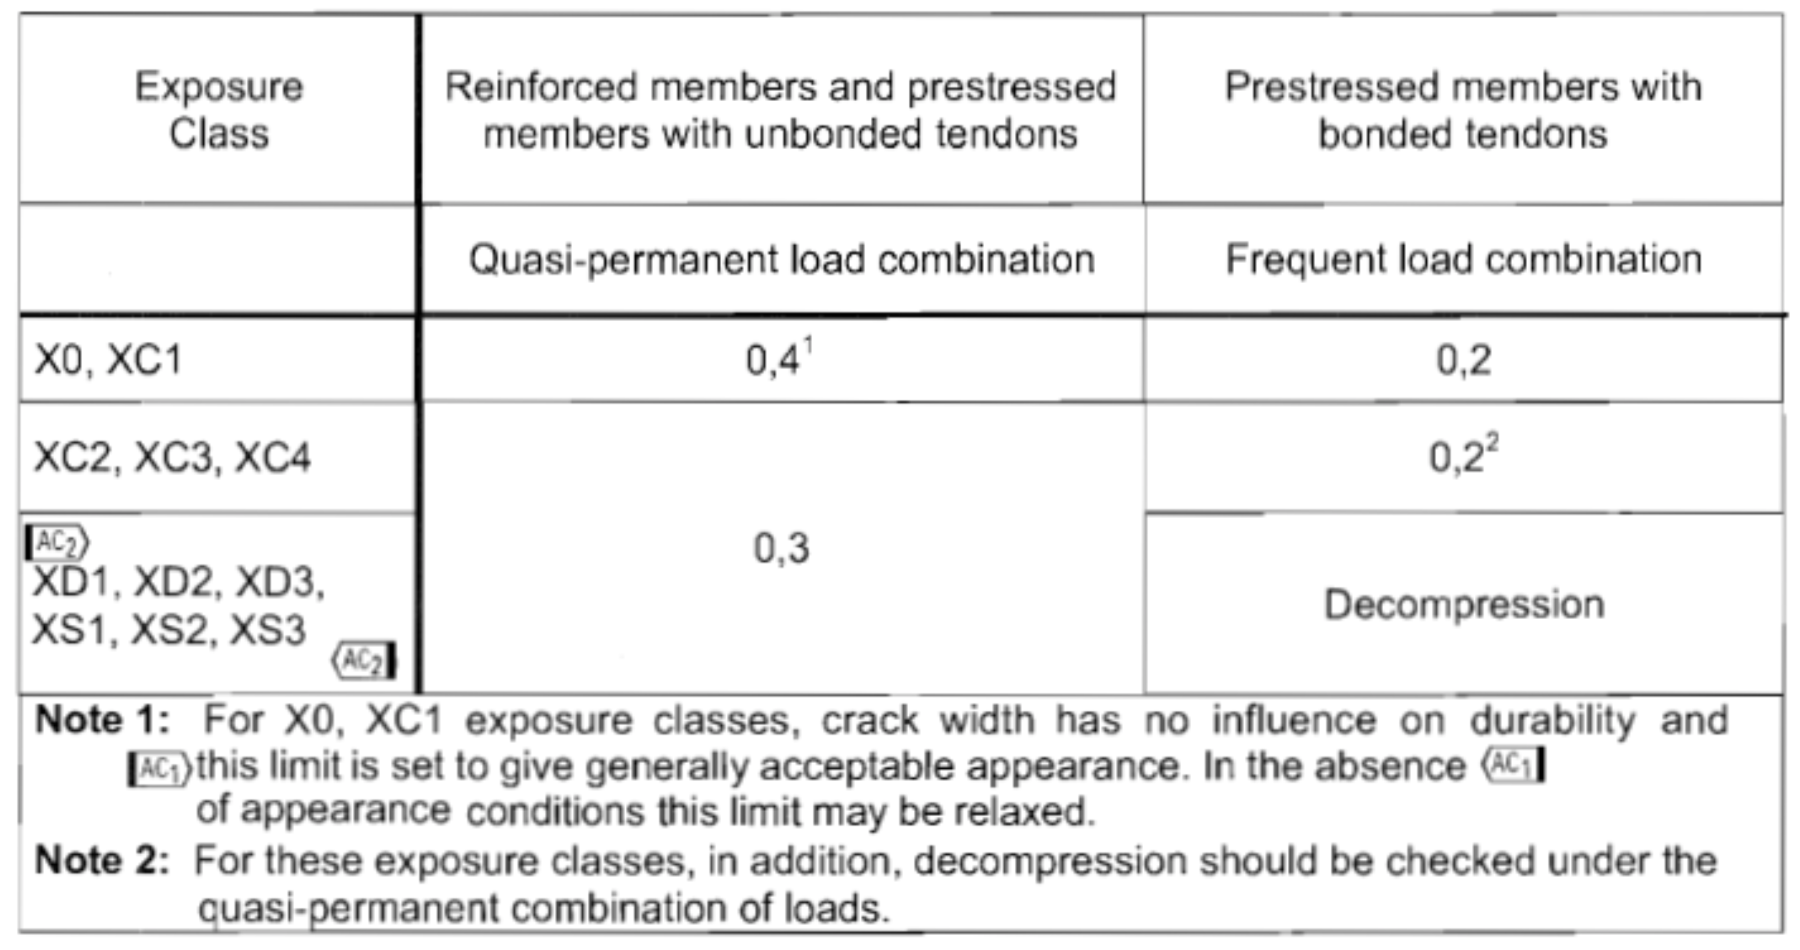
\includegraphics[width=0.8\linewidth]{img/7_1.png}
    \caption{Maximum allowable crack width depending on technology and environmental conditions}
    \label{tab:max_crack}
\end{table}

\begin{table}[H]
  \centering
  \begin{tabular}{cccc}
    \toprule
      $\omega = 0,2$ [mm] & $\omega = 0,3$ [mm] & $\omega = 0,4$ [mm] & Máxima tensión $\sigma$ [Mpa]\tabularnewline
    \midrule
      25 & 32 & 40 & 160\tabularnewline
      16 & 25 & 32 & 200\tabularnewline
      12 & 16 & 20 & 240\tabularnewline
      8 & 12 & 16 & 280\tabularnewline
      6 & 10 & 12 & 320\tabularnewline
      5 & 8 & 10 & 360\tabularnewline
      4 & 6 & 8 & 400\tabularnewline
      - & 5 & 6 & 450\tabularnewline
    \bottomrule
  \end{tabular}
  \caption{Diámetro (en $mm$) de barra en función $\sigma_{max}$ y $\omega$}
  \label{tab:tension_grieta}
\end{table}

\begin{table}[H]
  \centering
  \begin{tabular}{cccc}
    \toprule
      $\omega = 0,2$ [mm] & $\omega = 0,3$ [mm] & $\omega = 0,4$ [mm] & Máxima tensión $\sigma$ [Mpa]\tabularnewline
    \midrule
      200 & 300 & 300 & 160\tabularnewline 
      150 & 250 & 300& 200\tabularnewline  
      100 & 200 & 250 & 240\tabularnewline
      30 & 150 & 200 & 280\tabularnewline
      - & 100 & 150 & 320\tabularnewline
      - & 50 & 100 & 360\tabularnewline
    \bottomrule
  \end{tabular}
  \caption{Spacing (en $mm$) en función $\sigma_{max}$ y $\omega$}
  \label{tab:spacing_grieta}
\end{table}
% subsection reinforced (end)

\subsection{Prestressed} % (fold)
\label{sub:prestressed}
We need to find $(P,e)$ that fullfills:
    \begin{gather}\label{eq:2.1}
      \begin{cases}
        \sigma_{comp,const} = \frac{P}{A} - \frac{P e \nu_t}{I} + \frac{M_g \nu_t}{I} \leq \sigma_{max,comp}=0,6fck\\
        \sigma_{trac,const} = -\frac{P}{A} + \frac{P e \nu_t}{I} + \frac{M_g \nu}{I} \leq \sigma_{max,trac}=3MPa\\
        \sigma_{comp} = \frac{P}{A} - \frac{P e \nu_t}{I} + \frac{M_{characteristic} \nu_t}{I} \leq \sigma_{max,comp}=0,6fck\\
        \sigma_{trac} = -\frac{P}{A} + \frac{P e \nu_t}{I} + \frac{M_{frequent} \nu}{I} \leq \sigma_{max,trac}=3MPa
      \end{cases}\\
      \shortintertext{where}
      \begin{aligned}
        &\nu: \emph{ is the distance to the c.g from the bottom} \\
        &\nu_t: \emph{ is the distance to the c.g from the top} \\
        &\emph{Signs }\emph{we suposed the resulting moments compress the top and prestressed ones the bottom} \\
        & M_g: \emph{ is the moment in a construction phase}
      \end{aligned}\notag
    \end{gather}
% subsection prestressed (end)

% section crack_width_control (end)

\section{Shear reinforcement} % (fold)
\label{sec:shear_reinforcement}
Procedure:
\begin{enumerate}
  \item Compute $V_d$

  \item Compute

    \begin{gather}\label{eq:2.1}
      V_c = \max
      \begin{cases}
        V_{R_d,c} = \left(C_{Rd,c}k(100\rho_l f_{ck})^{1/3}+k_1 \sigma_{cp}\right)b_wd\\
        V_{R_d,c,min}=\left(0,035 \cdot k^{3/2}f_{ck}^{1/2}+k_1 \sigma_{cp}\right)b_wd
      \end{cases}\\
      \shortintertext{where}
      \begin{aligned}
        &C_{Rd,c} = \frac{0,18}{\gamma_c} = 0,12 \\
        &k = 1 + \sqrt{\frac{200}{d}}\leq 2 \emph{ in mm} \\
        &\rho_l = \frac{A_{s,long}}{b_w d } \leq 0,02 \\
        &k_1 = 0,15\\
        &\sigma_{cp} = \frac{N+P}{b_w d}\leq 0,2 f_{cd}
      \end{aligned}\notag
    \end{gather}
    \item If $V_d>V_c \rightarrow$ reinforcement needed

  \item Compute 

    \begin{gather}\label{eq:1.2}
      V_{R_d,max} = a_{cw} b_w z \nu_1 f_{cd} \frac{1}{\cot(\theta) + \tan(\theta)}\\
      \shortintertext{where}
      \begin{aligned}
        &\nu_1 = 
          \begin{cases}
            0,6 &\text{ if } f_{ck} \leq 60 MPa\\
            0,9 - \frac{f_{ck}}{200}>0,5 & \text{ if } f_{ck} > 60 MPa
          \end{cases} \\
        &\alpha_{cw} = 
          \begin{cases}
            1 & \emph{non prestressed structure}\\
            1+ \sigma_{cp}/f_{cd} - \frac{f_{ck}}{200}>0,5 & \text{ if } \sigma_{cd} \leq 0,25 f_{cd} \\
            1,25 & \text{ if } 0,25f_{cd} <\sigma_{cd} \leq 0,5 f_{cd} \\
            2,5 (1- \sigma_{cp}/f_{cd}) & \text{ if } 0,5f_{cd} <\sigma_{cd} \leq f_{cd}
          \end{cases} \\
        & z \approx 0,9 d \approx 0,8 h \\
        & \cot(\theta) = 2,5
      \end{aligned}\notag
    \end{gather}

  \item If $V_{R_d,max}< V_d$
    \begin{enumerate}
      \item Compute 
      \[
        \nu = \frac{V_d}{a_{cw} b_w z \nu_1 f_{cd}}
      \]
      \item If $\nu > 0,5$ increase $b_w$ or $z$, and/or $f_{cd}$
      \item 
      \begin{equation}
        \cot(\theta) = 
          \begin{cases}
            2,5 &\text{ if } \nu \leq 0,34\\
            5,6 - 9,2 \nu & \text{ if } \nu > 0,34
          \end{cases}\in [1,2.5]
      \end{equation}
    \end{enumerate}
  \item Compute
    \begin{gather}\label{eq:1.3}
        \frac{A_{sw}}{s}= \frac{V_d}{f_{ywd}z \cot(\theta)}\\
        \shortintertext{where}
        \begin{aligned}
          & f_{ywd} = \min(\frac{f_{ywk}}{\gamma_s},400)
        \end{aligned}\notag
      \end{gather}

  \item If $\frac{A_{sw}}{s} < \frac{A_{sw,min}}{s} = \frac{0,08 \sqrt{f_{ck}}}{f_{ywd}b_w}$

  \[
    \frac{A_{sw}}{s}=\frac{A_{sw,min}}{s}
  \]

  \item Define 

    \begin{gather}\label{eq:1.4}
        A_{sw}= n \frac{\phi^2}{4}\\
        \shortintertext{where}
        \begin{aligned}
          & \phi: \emph{ is the diameter of the bars, see Table~\ref{tab:diam_tran}}\\
          & n: \emph{ the number of bars along the height of the section}\\
          & \emph{ it should be choosed in order to have $s_{section}<500mm$}
        \end{aligned}\notag
    \end{gather}

  \item Compute the spacing $s$
\end{enumerate}

\begin{table}[H]
  \centering
  \begin{tabular}{cc}
  \toprule
  Diameter [$mm$] & Area [$mm^2$] \\
  \midrule
  6 & 28 \\
  8 & 50 \\
  10 & 78 \\
  12 & 113 \\
  \bottomrule
  \end{tabular}
  \caption{Common diameters for transversal reinforcement}
  \label{tab:diam_tran}
\end{table}
\subsection{Optimisation} % (fold)
\label{sub:optimisation}
Process
\begin{enumerate}
  \item Choose $x$
  \item Compute $V_{d,x+d}$
  \[
    n=\frac{V_{d,x+d}}{V_{d,max}}
  \]
  \item Compute $s_{x+d} = n s_{min}$
\end{enumerate}
% subsection optimisation (end)
% section shear_reinforcement (end)

\section{Columns} % (fold)
\label{sec:columns}
\subsection{Second order effects} % (fold)
\label{sub:second_order_effects}
\begin{enumerate}
  \item Compute 
    \begin{gather}\label{eq:1.4}
        \varphi_{ef} = \frac{M_{quasi}}{M_d}\varphi\\
        \shortintertext{where}
        \begin{aligned}
          & \varphi: \emph{ is the creep coeficient}\\
          & M_{quasi}: \emph{ the quasi-permanent combination (realistic load case)}
        \end{aligned}\notag
    \end{gather}
  \item Compute 
    \begin{gather}\label{eq:1.4}
        E_{cd}I_{cd} = \frac{0,3}{1+ \varphi_{ef}}E_{cd}I_c\\
        \shortintertext{where}
        \begin{aligned}
          & E_{cd} = \frac{E_c}{1,2}\\
          & I_c = I_{gross}
        \end{aligned}\notag
    \end{gather}
  \item Compute $L_p$, see Figure~\ref{fig:buck}
  \item Compute $N_B = \left(\frac{\pi}{L_p}\right)^2E_{cd}I_{cd}$
  \item Compute
  \begin{equation}
    M_{d,2} = \frac{M_d}{1 - \frac{N_d}{N_B}}
  \end{equation}
\end{enumerate}
\begin{figure}[H]
    \centering
    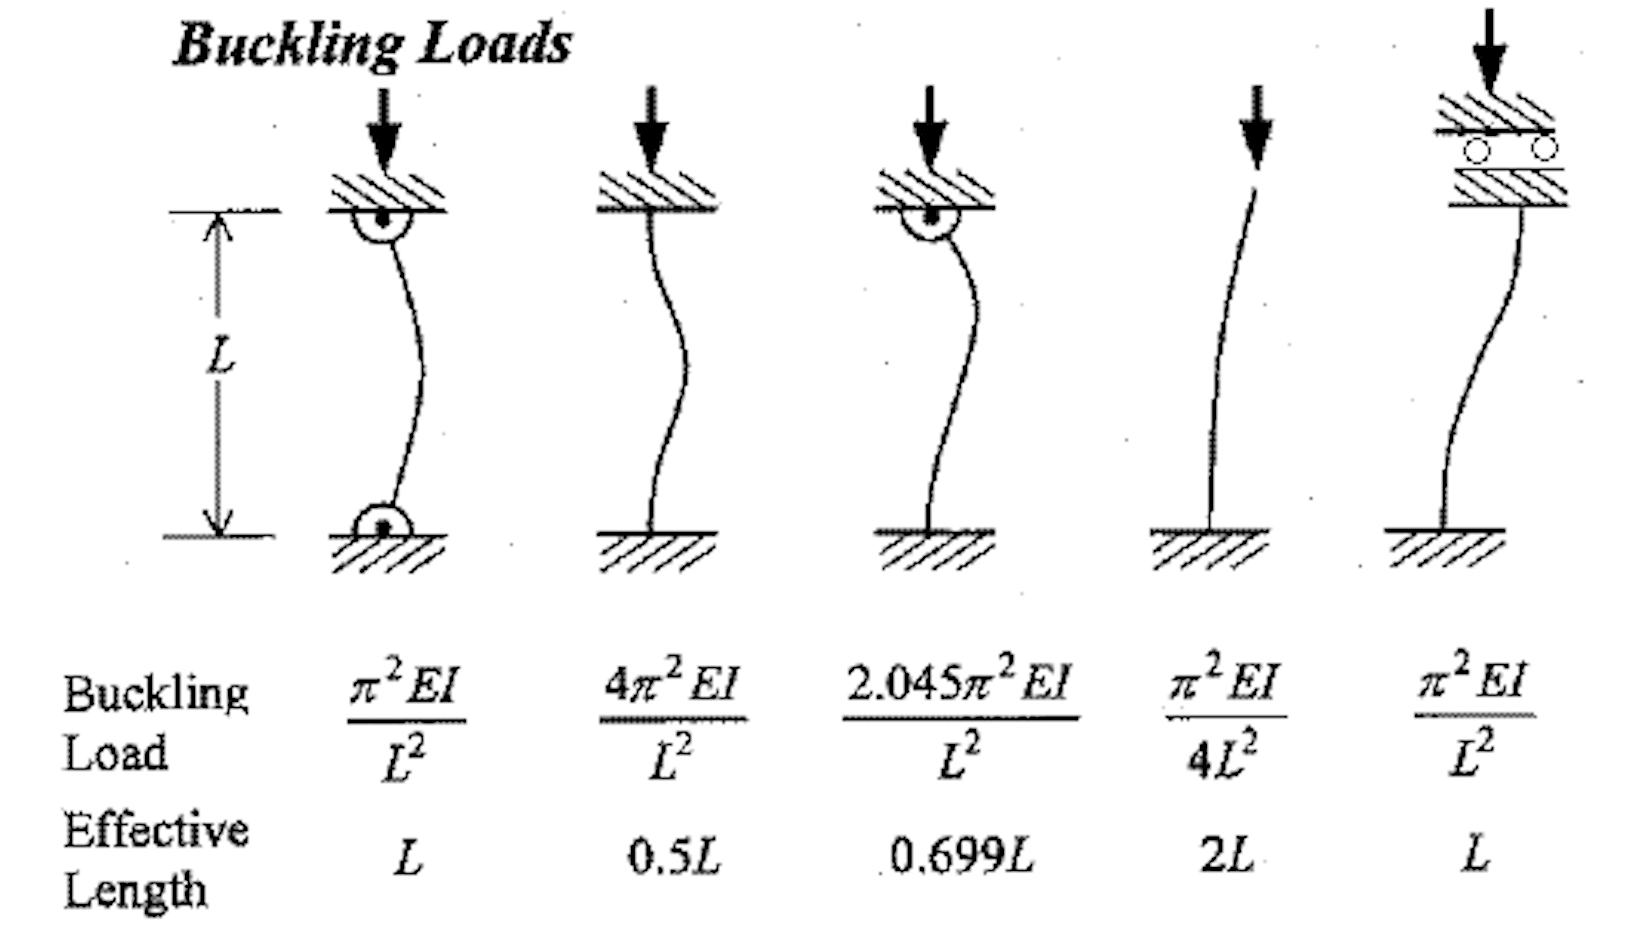
\includegraphics[width=0.95\linewidth]{img/buckling}
    \caption{Buckling length and load depending on the support}
    \label{fig:buck}
\end{figure}

  \subsection{Longitudinal reinforcement} % (fold)
  \label{sub:longitudinal_reinforcement}
  \begin{enumerate}
    \item Compute $\nu = \frac{N_d}{A_c f_{cd}}$
    \item Compute $\mu = \frac{M_{d,2}}{A_c D f_{cd}}$\\
    where $D:\emph{ is a charasteristic length}$
    \item Find $w (\nu, \mu) = \frac{A_s f_{yd}}{A_c f_{cd}}$
    \item Check minimal quantity
    \[
      w = \max(w;w_{min}=0,01)
    \]
  \end{enumerate}

  \subsection{Transversal reinforcement} % (fold)
  \label{sub:transversal_reinforcement}
  \begin{enumerate}
    \item Compute 
    $\tau_c = \frac{V_c}{bd}$
    \item If $\tau_c<0,5 MPa$ (can be resisted by concrete we should put the minimum)
    \begin{equation}
      \begin{cases}
        \phi_{t}>\phi_{min} = \frac{\phi_{long}}{4}\\
        s_{t}< 15 \phi_{long}
      \end{cases}
    \end{equation}
  \end{enumerate}

  \section{Detailing and layout} % (fold)
  \label{sec:detailing_and_layout}
  \begin{itemize}
    \item Along the section the maximal distance between bar axes should be $d_{max}=300mm$
  \end{itemize}
  % section detailing_and_layout (end)
  
  % subsection transversal_reinforcement (end)
  % subsection longitudinal_reinforcement (end)

% subsection second_order_effects (end)
% section columns (end)
\newpage

\addcontentsline{toc}{section}{Bibliografia}
\nocite{*}
\printbibliography
\end{multicols*}


\end{document}
